\section{Authentication}

\subsection{Sign in Page and Process}

\noindent Sign in Page and Process

\vspace{0.3cm}

\noindent The system needs to make sure that users are really who they say they are. This is a security check to keep everything. It makes sure that authorized people can use the features of the sign in page and process.

\vspace{0.3cm}

\noindent The system has a sign in process that all users need to follow. This includes students, administrators and office staff who all have to sign in.

\vspace{0.3cm}

\noindent The sign in process is very easy to use. It works well for everyone. The sign in page and process are available in two languages: English and Bengali.

\vspace{0.3cm}

\noindent The sign in page looks modern and clean which makes it easy to use the sign in page and process.

\vspace{0.3cm}

\noindent Here's how to sign in to the sign in page and process:

\begin{itemize}
    \item \textbf{Enter your details:} You need to enter your ID and password on the sign in page. Students can use their email or GST Admission Roll on the sign in page. The initial password for students is their HSC Roll, which they use on the sign in page.

    \item \textbf{See your password:} There is a button that lets you view what you type on the sign in page. This helps you check and avoid mistakes on the sign in page.

    \item \textbf{Login:} You click the Login button on the sign in page. This starts the verification process for the sign in page and process.

    \item \textbf{Go to your page:} If you sign in correctly to the sign in page the system takes you to your page. This could be the Student page, the Dean page or the Registrar page, which you can access after signing in to the sign in page and process.

    \item \textbf{Error:} If you sign in incorrectly to the sign in page the system does not let you in. It says that the username or password is incorrect for the sign in page and process.
\end{itemize}

\begin{figure}[htbp]
    \centering
    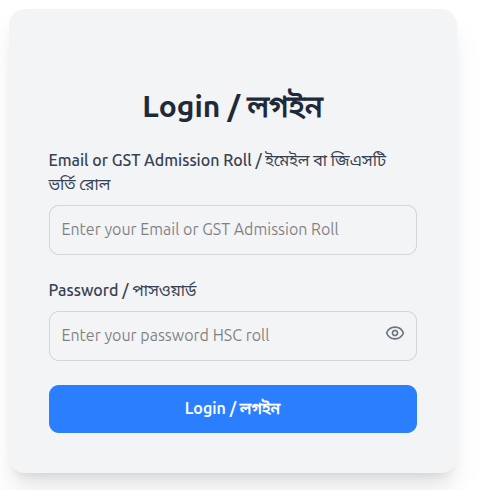
\includegraphics[width=0.6\textwidth]{chapters/chapter4/images/login.png}
    \caption{System Authentication (Login Page)}
    \label{fig:authentication_login}
\end{figure}